\skriptsection{Complexe Zahlen}{1}
\skriptsubsection{Grundlagen}{1ff}
\begin{minipage}[t]{9.4cm}
  \textbf{Cartesische Form}\\
  Normalform: $z = z_1 +j z_2$\\
  $z_1 = \text{Re}(z), \quad z_2 = \text{Im}(z)$\\
  Umrechnung in Polar:\\
  $r = |z| = \sqrt{z_1^2 + z_2^2}, \quad 
  \varphi =   \begin{cases} 
                  \arctan(\frac{z_2}{z_1}) &z_1 \geq 0\\
                  \arctan(\frac{z_2}{z_1}) + \pi &z_1 < 0
          \end{cases}$
\end{minipage}
\begin{minipage}[t]{9.4cm}
  \textbf{Polarsystem}\\
  Normalform: 
  $z = r \cjs(\varphi) = r(\cos{\varphi} + j\sin{\varphi}) = r e^{j \varphi}$\\
  $\varphi = \arg(z)$

  Umrechnung in Cartesisch:\\
  $z_1 = |z| \cos{\varphi}, \quad z_2 = |z| \sin{\varphi}$
\end{minipage}
\begin{center}
{\textbf{Imaginäre Einheit} $\qquad j^2 = -1 \qquad e^{j\pi} = -1 \qquad
\frac{1}{j} = -j$}
\end{center}

\skriptsubsection{Rechenregeln}{10ff}
\begin{tabular}{ll}
$+, -$
&Selbige Regeln wie für $\mathbb{R}$\\

Mulitplikation
&$a \cdot b = 
|a| |b| \cjs(\alpha + \beta) = 
|a| |b| e^{j(\alpha + \beta)}$\\

Division
&$\left|\frac{a}{b}\right| = 
\frac{\left|a\right|}{\left|b\right|} \cjs(\alpha - \beta) =
\frac{\left|a\right|}{\left|b\right|} e^{j(\alpha - \beta)}$ (cartesisch: Mit
conj. complex des Nenners erweitern) \\

Conjugiert complex
&$\overline{z} = \overline{z_1 + jz_2} = z_1 - jz_2; \qquad \qquad z \cdot \overline{z} = |z|^2$\\

Wurzeln
&$\sqrt[n]{a} = \sqrt[n]{|a|} \cjs(\frac{arg(a)}{n}+k\frac{2\pi}{n}) = 
\sqrt[n]{|a|} e^{j(\frac{\alpha}{n} + k \frac{2\pi}{n})} \quad (k = 0, 1,
\ldots, n-1 \Rightarrow \text{n Lösungen in } \mathbb{C} !)$ \\

Potenzen
&$a^n = |a|^n \cjs(n\alpha) = 
|a|^n e^{jn\alpha}$\\

$e^z$ &$e^{z_1+jz_2} = e^{z_1} \cjs(z_2) = e^{z_1} (\cos{z_2} + j\sin{z_2})$\\

Moivre'sche Formel
&$\text{cjs}^n(\varphi) =
(\cos{\varphi} + j\sin{\varphi})^n = 
\cos(n\varphi) +j\sin(n\varphi) \quad (n \in \mathbb{N})$\\

Logarithmus
&$Ln(z) = \ln{|z|} + j (\arg(z) + 2k \pi)$
\end{tabular}

\begin{minipage}[t]{11.4cm}
  \textbf{Bemerkungen}\\
  \begin{itemize}
    \item $p_n(z) \; (n \geq 1, z \in \mathbb{C})$ hat $n$ Lösungen und Nullstellen (in
  $\mathbb{C}$)  
    \item Allgemeine Potenzen $a^b,\;a,b \in \mathbb{C}$ können mit $e^{b \cdot 
    Ln(a)}$ und den bekannten für $\mathbb{R}$ gültigen Potenzregeln gelöst
    werden.
    \item Re$\left (\frac{a}{b} \right) = 0$: Die beiden compl. Zahlen $a, b$
    stehen senkrecht zueinander.
  \end{itemize}
\end{minipage}
\begin{minipage}[t]{7.4cm}
  \textbf{Einheitswurzeln}\\
  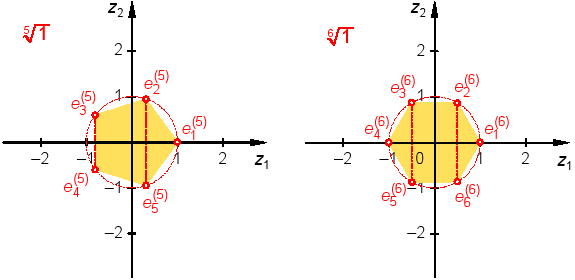
\includegraphics[width=7cm]{./bilder/einheitswurzel.png}
\end{minipage}
\subsection{12. Einheitswurzeln ($k 30 \symbol{23}$)}
$e^{(12)}_1 = 1,\;
  e^{(12)}_2 = \frac{\sqrt3}{2} + \frac12j,\;
  e^{(12)}_3 = \frac12 + \frac{\sqrt3}{2}j,\;
  e^{(12)}_4 = j,\;
  e^{(12)}_5 = -\frac12 + \frac{\sqrt3}{2}j,\;
  e^{(12)}_6 = -\frac{\sqrt3}{2} + \frac12 j,\\
  e^{(12)}_7 = -1,\;
  e^{(12)}_8 = -\frac{\sqrt3}{2} - \frac12 j,\;
  e^{(12)}_9 = -\frac12 - \frac{\sqrt3}{2}j,\;
  e^{(12)}_{10} = -j,\;
  e^{(12)}_{11} = \frac12 - \frac{\sqrt3}{2}j,\;
  e^{(12)}_{12} = \frac{\sqrt3}{2} - \frac12j$

\subsection{Nullstellen von Polynomen}
Ein complexes Polynom p(z) von Grad $n$ hat in $ \mathbb{C} $ genau $n$ Nullstellen.\\
Alle diese Nullstellen liegen in einer Kreisscheibe um den Ursprung mit dem Radius $ \sum\limits_{k=0}^{n} \left| \frac{a_k}{a_n} \right|$ \\ \\
Bei Polynomen mit reellen Koeffizienten treten nicht-reelle Nullstellen immer
als conj.-compl. Paare ($z_0$ und $\bar{z_0}$) auf. 

\skriptsubsection{Euler}{30f}
\begin{tabular}{llllll}
$\sin{\alpha} = \frac{e^{j\alpha} - e^{-j\alpha}}{2j}$ &

$\cos{\alpha} = \frac{e^{j\alpha} + e^{-j\alpha}}{2}$ &

$\tan{\alpha} = \frac{\sin \alpha}{\cos \alpha}$ & 

$ \qquad \qquad $ &

$\sinh{\alpha} = \frac{e^\alpha - e^{-\alpha}}{2} $ &

$\cosh{\alpha} = \frac{e^\alpha + e^{-\alpha}}{2} $
\end{tabular}

\skriptsubsection{Überlagerung von harmonischen Schwingungen}{32f}
$$A \cdot \sin(\omega t + \varphi) = Im[A \cdot e^{j(\omega t + \varphi)}] =
Im[\underbrace{A \cdot e^{j\varphi}}_{\text{\tiny{Complexe Amplitude}}}
\cdot \underbrace{e^{j\omega t}}_{\text{\tiny{Zeitfunktion}}}]$$
%
%Alle komplexen Schwingungen in kartesische Form umwandeln und addieren, danach
%wieder zurück in Polarform $ A_{total} \cdot e^{j\varphi}$ zurückwandeln.
%
$$ A_1 \cdot \sin(\omega t + \varphi_1) + A_2 \cdot \cos(\omega t + \varphi_2) 
 \quad \Rightarrow \quad 
 Im[A_1 \cdot e^{j(\omega t + \varphi_1)} + A_2 \cdot e^{j (\omega t + \varphi_2
 + \frac{\pi}{2})}] \quad \Rightarrow \quad 
 Im[e^{j \omega t} \cdot  (A_1 \cdot e^{j \varphi_1} + A_2 \cdot e^{j (\varphi_2
 + \frac{\pi}{2})}]$$ 
Complexe Amplituden in cartesische Form umwandeln, zusammenzählen und wieder
zurück in Polarform wandeln.
$$ Im[e^{j \omega t} \cdot  (A_{total} \cdot e^{j \varphi_{total}})] 
 \quad \Rightarrow \quad 
 Im[A_{total} \cdot e^{j (\omega t + \varphi_{total})}] 
 \quad \Rightarrow \quad 
 A_{total} \cdot \sin(\omega t + \varphi_{total})$$

%Bsp: 
%$y = y_1 + y_2 = A_1 \sin(\omega t + \varphi_1) + A_2 \underbrace{\cos(\omega t
%+ \varphi_2)}_{\text{\tiny{zu sin verwandeln}}}
%= A_1 \sin(\omega t + \varphi_1) - A_2 \sin(\omega t + (\varphi_2
%-\frac{\pi}{2}))$\\
%$= \text{Im}(\underbrace{A_1 e^{j\varphi_1}}_{\text{\tiny{$A_{1im} = A_1 \cjs
%A_1 \cdot \sin(\omega t + \varphi_1) + \varphi_1$}}} e^{j\omega t} - 
%\underbrace{A_2 e^{j(\varphi_2 - \frac{\pi}{2})}}_{\text{\tiny{$A_{2im} = A_2 \cjs
%(\varphi_2 - \frac{\pi}{2})$}}} e^{j \omega t}) 
%= (A_{1im} + A_{2im}) \sin(\omega t)$